\documentclass[aspectratio=169, table]{beamer}

\usepackage[utf8]{inputenc}
\usepackage{listings} 

\usetheme{Pradita}

\subtitle{MTI104 - IT Services}

\title{Session-05:\\\LARGE{Influencing Through Guiding \\Principles}}
\date[Serial]{\scriptsize {PRU/SPMI/FR-BM-18/0222}}
\author[Pradita]{\small{\textbf{Alfa Yohannis}}}

\begin{document}

\frame{\titlepage}

\begin{frame}
	\frametitle{Guiding Principles Overview}
	\begin{itemize}
		\item Guiding principles are boundaries within which you can operate.
		\item They are recommendations, not rules or policies.
		\item ITIL's nonprescriptive nature is a key strength.
		\item The concept of guiding principles is new to ITIL.
		\item Introduced in 2016 with ITIL Practitioner certification.
		\item Initially, there were nine guiding principles.
		\item In ITIL 4, the principles have been revamped into seven.
	\end{itemize}
\end{frame}

\begin{frame}
	\frametitle{The Seven Guiding Principles of ITIL}
	\begin{itemize}
		\item Focus on Value
		\item Start Where You Are
		\item Progress Iteratively with Feedback
		\item Collaborate and Promote Visibility
		\item Think and Work Holistically
		\item Keep it Simple and Practical
		\item Optimize and Automate
	\end{itemize}
\end{frame}

\begin{frame}
	\frametitle{Importance in ITIL Foundation Exam}
	\begin{itemize}
		\item Guiding principles are crucial for the ITIL Foundation exam.
		\item You can expect five questions on guiding principles.
		\item These principles account for 12.5\% of the total exam questions.
		\item Questions test understanding and application of principles.
		\item Important to know the context of each guiding principle.
		\item The guiding principles are universal and practical.
		\item They are aligned with the Agile manifesto.
	\end{itemize}
\end{frame}

\begin{frame}
	\frametitle{Application Across Industries}
	\begin{itemize}
		\item Guiding principles apply to all industries, not just ITIL.
		\item They are common sense but need constant reinforcement.
		\item Similarities with Agile manifesto:
		\item Focus on Value aligns with Agile's "working software over documentation".
		\item Responding to change aligns with "Progress Iteratively with Feedback".
		\item Organizations may combine different methodologies.
	\end{itemize}
\end{frame}

\begin{frame}
	\frametitle{Combining Frameworks}
	\begin{itemize}
		\item Guiding principles allow integration of various frameworks.
		\item Agile methodology focuses on project flexibility.
		\item DevOps integrates development (Agile) and operations (ITIL).
		\item Prioritization conflicts can arise in integrated teams.
		\item Guiding principles provide direction in such conflicts.
		\item Example: Prioritizing tasks based on value creation.
		\item Frameworks like Prince, Lean, COBIT can align under common principles.
	\end{itemize}
\end{frame}

\begin{frame}
	\frametitle{Implementation and Relevance}
	\begin{itemize}
		\item Organizations should not selectively apply guiding principles.
		\item All seven guiding principles come as a set.
		\item Practical to use relevant principles based on context.
		\item Contextual application is crucial for effectiveness.
		\item Focus on Value is central to ITIL.
		\item It directs activities toward creating value for customers.
		\item Organizations must link services to value generation.
	\end{itemize}
\end{frame}

\begin{frame}
	\frametitle{Focus on Value}
	\begin{itemize}
		\item ITIL emphasizes creating value for the customer.
		\item Every service activity should link back to value creation.
		\item Example: Netflix gathers data to enhance customer value.
		\item Netflix uses customer data to fund and recommend new shows.
		\item Value creation benefits all stakeholders, not just customers.
		\item Value generation follows a four-step process:
		\item Understand the service consumer, their perspective, obtain feedback, and apply learnings.
	\end{itemize}
\end{frame}

\begin{frame}
	\frametitle{Understanding the Service Consumer}
	\begin{itemize}
		\item Understanding consumer needs is essential for value creation.
		\item Service providers must know their customers deeply.
		\item Example: A Mexican restaurant targets neighborhoods that prefer spicy food.
		\item Service providers should also understand other stakeholders.
		\item Knowing consumer perspectives translates to valuable insights.
		\item Providers should explore the reasons behind service use.
		\item Value is about perception, not just service quality.
	\end{itemize}
\end{frame}

\begin{frame}
	\frametitle{Obtaining and Applying Feedback}
	\begin{itemize}
		\item Feedback is crucial in the service industry.
		\item CX (Customer Experience) reflects customer feelings toward a service.
		\item Feedback helps adjust to changing customer perceptions.
		\item Surveys and interactions gauge customer satisfaction.
		\item Feedback should lead to actionable insights.
		\item Applying feedback is essential for continuous improvement.
		\item Service providers must co-create value with customers.
	\end{itemize}
\end{frame}

\begin{frame}
	\frametitle{Start Where You Are}
	\begin{itemize}
		\item Start with the current state rather than starting anew.
		\item Reuse existing foundations instead of laying new ones.
		\item Assess the current state objectively before making changes.
		\item Measurements are key to understanding the current situation.
		\item Measure outcomes, not just outputs.
		\item Avoid the trap of biased assessments.
		\item Use measurements to inform decisions about future actions.
	\end{itemize}
\end{frame}

\begin{frame}
	\frametitle{Applying the Principle of Start Where You Are}
	\begin{itemize}
		\item Apply learnings from assessments to make informed decisions.
		\item Example: Modernizing a website with new features.
		\item Assess existing elements like CMS, server, and security.
		\item Identify what works and what doesn’t.
		\item Assess risks associated with current and new systems.
		\item Make decisions based on thorough analysis and risk assessment.
		\item Reuse what is functional; change what is necessary.
	\end{itemize}
\end{frame}

\begin{frame}{Applying the principle of start where you are}
	 \frametitle{ Applying the principle of start where you are}
\begin{center}
	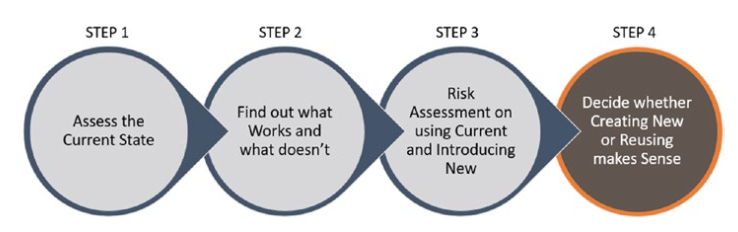
\includegraphics[width=0.8\linewidth]{images/image-01.png}
\end{center}
\end{frame}

\begin{frame}
	\frametitle{Applying the Principle of Start Where You Are}
\begin{itemize}
	\item Iterations and feedback are essential techniques.
	\item Minimum Viable Product (MVP) is a key method.
	\item MVP involves building with minimal configuration.
	\item Invest fewer resources for valuable feedback.
	\item Example: Online banking system with basic functionalities.
	\item MVP helps alter product development course.
	\item Ensures alignment with customer preferences.
\end{itemize}
\end{frame}

\begin{frame}{Feedback feeding iteration}
	 \frametitle{ Feedback feeding iteration}
\begin{center}
	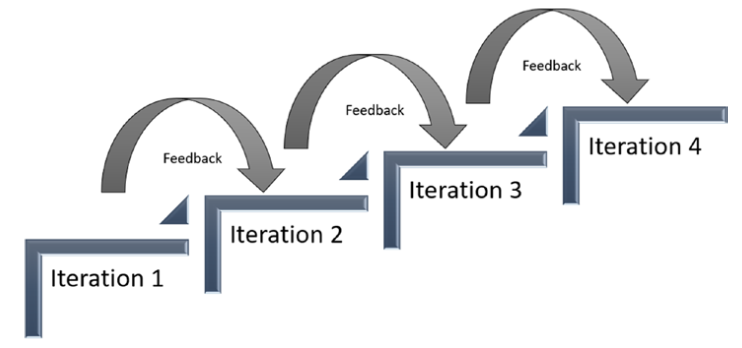
\includegraphics[width=0.8\linewidth]{images/image-02.png}
\end{center}
\end{frame}

\begin{frame}
\frametitle{Understanding MVP and Iterations}

\begin{itemize}
	\item Iterations don't mean quicker development.
	\item MVP doesn't imply releasing incomplete products.
	\item Products can be broken into functionalities.
	\item Develop functionalities in time-boxed periods.
	\item MVP includes the minimum set of required functionalities.
	\item Focus on the end product's final objective.
	\item Customer representatives keep tabs on progress.
\end{itemize}
\end{frame}

\begin{frame}
\frametitle{Avoiding Development Traps}

\begin{itemize}
	\item One common trap: "develop once, develop right."
	\item Deep analysis can lead to "analysis paralysis."
	\item Time-boxing is essential for all team activities.
	\item Non-core developmental efforts must also be time-boxed.
	\item Avoid over-analysis to maintain development pace.
	\item Focus on continuous progress and delivery.
	\item Balance between analysis and execution.
\end{itemize}
\end{frame}

\begin{frame}
\frametitle{Collaborate and Promote Visibility}

\begin{itemize}
	\item Collaboration, cooperation, and visibility drive Agile and DevOps.
	\item Team collaboration is crucial for success.
	\item Work must be transparent to customers.
	\item Product owners should be part of the development team.
	\item Involvement of customers in daily activities is necessary.
	\item Move away from siloed working environments.
	\item Promote shared knowledge and decision-making.
\end{itemize}
\end{frame}

\begin{frame}
\frametitle{Collaboration Partners}

\begin{itemize}
	\item Multiple service providers must work together.
	\item Trade secrets can hinder collaboration.
	\item Sharing skill sets can benefit all parties.
	\item Collaboration with customers is crucial.
	\item Customers should be involved at all project levels.
	\item Open collaboration between service providers and customers.
	\item Emphasize common goals for better delivery.
\end{itemize}
\end{frame}

\begin{frame}
\frametitle{Means of Communication}

\begin{itemize}
	\item DevOps requires frequent conversations and visibility.
	\item Remote work challenges collaboration.
	\item Utilize tools like MS Teams, Slack, Google Meet.
	\item Video calling, group chats, and boards enhance collaboration.
	\item Move away from emails for routine communication.
	\item Use surveys to gather feedback from general users.
	\item Continuous feedback is central to improvements.
\end{itemize}
\end{frame}

\begin{frame}
\frametitle{Expanding Visibility}

\begin{itemize}
	\item Lack of visibility hinders team spirit and loyalty.
	\item Leaders must spread messages of organizational activities.
	\item Visibility is crucial in product/service development.
	\item Poor visibility causes customer panic and delays.
	\item Continuous communication ensures timely delivery.
	\item Agile frameworks support visibility and communication.
	\item Visibility impacts decision-making and direction.
\end{itemize}
\end{frame}

\begin{frame}
\frametitle{Applying the Principles/Learnings}

\begin{itemize}
	\item Collaboration and visibility are key learning points.
	\item Focus on work visibility across the organization.
	\item Decision-making must not be hindered by poor visibility.
	\item Collaboration is vital in remote working environments.
	\item Communication takes up a significant portion of project time.
	\item Identify the right types of communication for each scenario.
	\item Feedback must be embraced wisely and used effectively.
\end{itemize}
\end{frame}

\begin{frame}
\frametitle{Think and Work Holistically}

\begin{itemize}
	\item No product/service stands alone in delivering value.
	\item Think about connected systems and holistic approaches.
	\item Consider the impact on all related services and stakeholders.
	\item Integrations increase complexity and require careful planning.
	\item Collaboration and visibility are key to managing complexity.
	\item Automation helps manage repetitive tasks and reduce errors.
	\item Set clear principles and processes for a unified direction.
\end{itemize}
\end{frame}

\begin{frame}
\frametitle{Keep it Simple and Practical}

\begin{itemize}
	\item Minimalism is key to achieving objectives efficiently.
	\item Lean transformation guides resource optimization.
	\item Focus on outcomes that meet objectives with minimal steps.
	\item Remove waste, automate, and reduce bureaucracies.
	\item Avoid adding unnecessary controls at every step.
	\item Balance between oversight and efficiency.
	\item Practicality is essential in decision-making and execution.
\end{itemize}
\end{frame}

\begin{frame}
\frametitle{What to Shelve, What to Keep}

\begin{itemize}
	\item Identify wasteful activities and services through analysis.
	\item Avoid overburdening processes with unnecessary reviews.
	\item Streamline validation processes for smooth workflow.
	\item Example: Government tracking of cash transactions.
	\item Introduce conflict-free solutions for compliance.
	\item Automated validations reduce overhead.
	\item Focus on creating effective service management designs.
\end{itemize}
\end{frame}

\begin{frame}
\frametitle{Enablers to Simplicity and Pragmatism}

\begin{itemize}
	\item Enable systems to achieve 100\% compliance.
	\item Remove conflicts to encourage compliance.
	\item Example: Free Internet for online banking transactions.
	\item Ensure design considers inputs, players, triggers, and outcomes.
	\item Conflict-free designs are key to success.
	\item Change management requires balancing governance and operations.
	\item Automation and streamlined processes improve efficiency.
\end{itemize}
\end{frame}

\begin{frame}{Optimization and automation}
	 \frametitle{Optimization and automation}
\begin{center}
	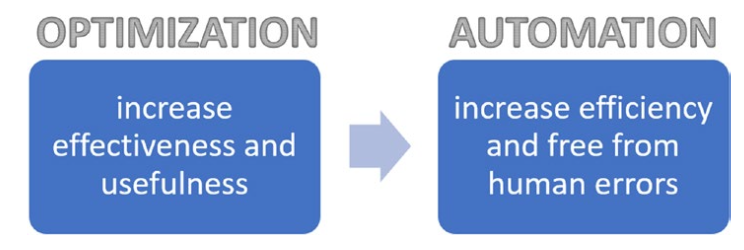
\includegraphics[width=0.8\linewidth]{images/image-03.png}
\end{center}
\end{frame}

\begin{frame}
	\frametitle{Question}
	
	Which of the following is the best definition of a guiding principle?
	
	\begin{itemize}
		\item[A.] A recommendation that guides an organization to set up a service management system
		\item[B.] A guide to build products and services
		\item[C.] A set of prescribed principles that provide direction to create value
		\item[D.] A recommendation that guides an organization in all circumstances
	\end{itemize}
	
\end{frame}


\end{document}
